\documentclass[t, aspectratio=169]{beamer}
\usetheme{Madrid}
\usecolortheme{default}
\usepackage[utf8]{inputenc}
\usepackage[T1]{fontenc}
\usepackage{graphicx}
\usepackage{tikz}
\usepackage[hypcap=true]{subcaption}
\usepackage{amsmath}
\usepackage{lmodern}
\usepackage[algo2e, ruled, vlined]{algorithm2e}

\usepackage[absolute,overlay]{textpos}
  \setlength{\TPHorizModule}{1mm}
  \setlength{\TPVertModule}{1mm}

  \resetcounteronoverlays{algocf}

\usepackage[
  backend       = biber, %biber does not work with 64x versions alternative: bibtex8
  %minalphanames only works with biber backend
  style=ieee,
  url = false,
  doi = false,
  ]{biblatex}

  \renewcommand\multicitedelim{\addsemicolon\space}

\addbibresource{../thesis/bibliography.bib}

\DeclareMathOperator*{\argmin}{arg\,min}

% Removes icon in bibliography
\setbeamertemplate{bibliography item}{}
\title[Lattice Parameter Estimation]{A Tool for the Estimation of Lattice Parameters}
\subtitle{Bachelor Thesis}
\author{Nicolai Krebs}
\date{November 26, 2021}

\AtBeginSection[]
{
  \begin{frame}
    \frametitle{Table of Contents}
    \tableofcontents[currentsection]
  \end{frame}
}

\tikzset{
  invisible/.style={opacity=0},
  visible on/.style={alt={#1{}{invisible}}},
  alt/.code args={<#1>#2#3}{%
    \alt<#1>{\pgfkeysalso{#2}}{\pgfkeysalso{#3}} % \pgfkeysalso doesn't change the path
  },
}

\begin{document}

\frame{\titlepage}
\begin{frame}
    \frametitle{Table of Contents}
    \tableofcontents
\end{frame}

\section{Motivation}
\begin{frame}
    \frametitle{Background}
    \begin{itemize}[<+->]
        \item Quantum computers can efficiently solve classically hard problems
              \begin{itemize}
                  \item Shor's algorithm (1994)\only<.->{\footfullcite{Shor97}}
                  \item Efficiently solves integer factorization problem % poly time
                  \item E.g., RSA becomes insecure
              \end{itemize}
        \item Different hardness assumptions needed
        \item[$\Rightarrow$] Lattice-based cryptography
    \end{itemize}
\end{frame}

\begin{frame}
    \frametitle{Lattice-based Cryptography}
    \begin{block}{Lattice}
        A lattice is a discrete $\Lambda$ additive subgroup of the vector space $\mathbb{R}^m$ and can be defined by a basis $\mathbf{B}$ of $n$ linearly independent vectors $\mathbf{b}_1, \ldots, \mathbf{b}_n \in \mathbb{R}^m$ with $m\geq n$.
    \end{block}\pause
    \begin{figure}
        \centering
        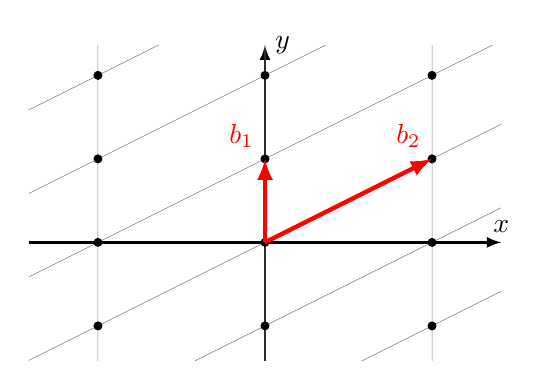
\begin{tikzpicture}[line/.style={>=latex}]
            \coordinate (Origin)   at (0,0);
            \coordinate (XAxisMin) at (-3,0);
            \coordinate (XAxisMax) at (3,0);
            \coordinate (YAxisMin) at (0,-1.5);
            \coordinate (YAxisMax) at (0,2.5);
            \draw [thick, black,-latex, visible on=<2->] (XAxisMin) -- (XAxisMax) node [above] {$x$};
            \draw [thick, black,-latex, visible on=<2->] (YAxisMin) -- (YAxisMax) node [right] {$y$};

            \clip (-3,-1.5) rectangle (3, 2.5);
            \pgftransformcm{1.41421356}{0.70710678}{0}{0.7071}{\pgfpoint{0cm}{0cm}}
            \coordinate (Bone) at (0,1.5);
            \coordinate (Btwo) at (1.5,0);
            \draw[style=help lines, visible on=<4->] (-14,-14) grid[step=1.5cm] (14,14);
            \foreach \x in {-7.5,-6.75,...,7}{
                    \foreach \y in {-7.5,-6.75,...,7}{
                            \node[draw,circle,inner sep=1pt,fill,, visible on=<3->] at (2*\x,2*\y) {};
                        }
                }
            \draw [ultra thick,-latex,red, visible on=<2->] (Origin)
            -- (Bone) node [above left] {$b_1$};
            \draw [ultra thick,-latex,red, visible on=<2->] (Origin)
            -- (Btwo) node [above left] {$b_2$};
        \end{tikzpicture}
        \caption{Lattice with basis $\mathbf{b}_1 = (0, 1)^\intercal,\; \mathbf{b}_2 = (2, 1)^\intercal$}
    \end{figure}
\end{frame}

\begin{frame}
    \frametitle{Lattice-based Cryptography}
    \begin{block}{Lattice}
        A lattice is a discrete $\Lambda$ additive subgroup of the vector space $\mathbb{R}^m$ and can be defined by a basis $\mathbf{B}$ of $n$ linearly independent vectors $\mathbf{b}_1, \ldots, \mathbf{b}_n \in \mathbb{R}^m$ with $m\geq n$.
    \end{block}
    \begin{figure}
        \centering
        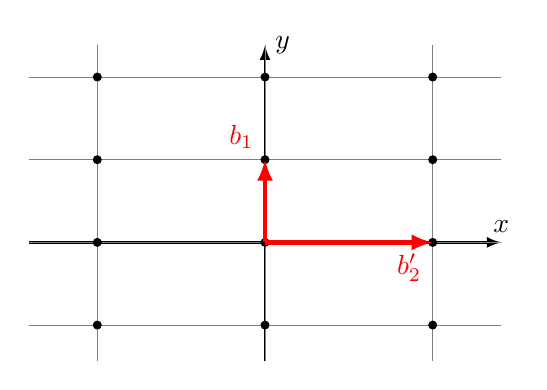
\begin{tikzpicture}[line/.style={>=latex}]
            \coordinate (Origin)   at (0,0);
            \coordinate (XAxisMin) at (-3,0);
            \coordinate (XAxisMax) at (3,0);
            \coordinate (YAxisMin) at (0,-1.5);
            \coordinate (YAxisMax) at (0,2.5);
            \draw [thick, black,-latex, visible on=<1->] (XAxisMin) -- (XAxisMax) node [above ] {$x$};
            \draw [thick, black,-latex, visible on=<1->] (YAxisMin) -- (YAxisMax) node [right] {$y$};

            \clip (-3,-1.5) rectangle (3, 2.5);
            \pgftransformcm{1.42}{0}{0}{0.7}{\pgfpoint{0cm}{0cm}}
            \coordinate (Bone) at (0,1.5);
            \coordinate (Btwo) at (1.5,0);
            \draw[style=help lines, visible on=<2->] (-14,-14) grid[step=1.5cm] (14,14);
            \foreach \x in {-7.5,-6.75,...,7}{
                    \foreach \y in {-7.5,-6.75,...,7}{
                            \node[draw,circle,inner sep=1pt,fill, visible on=<1->] at (2*\x,2*\y) {};
                        }
                }
            \draw [ultra thick,-latex,red] (Origin)
            -- (Bone) node [above left] {$b_1$};
            \draw [ultra thick,-latex,red] (Origin)
            -- (Btwo) node [below left] {$b_2'$};
        \end{tikzpicture}
        \caption{Lattice with basis $\mathbf{b}_1 = (0, 1)^\intercal,\; \mathbf{b}_2' = (2, 0)^\intercal$}
    \end{figure}
\end{frame}

\begin{frame}
    \frametitle{Lattice-based Cryptography}
    \begin{block}{SVP$_\gamma$ and \textsc{GapSVP}$_\gamma$}
        Given a basis $\mathbf{B}$ of a lattice $\Lambda$, the (approximate) Shortest Vector Problem (SVP$_\gamma$) is the problem of finding a short lattice vector $\mathbf{v}\in \Lambda$ such that $0 < \|\mathbf{v} \| \leq \gamma \lambda_1(\Lambda)$. The corresponding decision version is the \textsc{GapSVP}$_\gamma$ problem, in which we are asked to decide whether $\lambda_1(\Lambda) \leq 1$ or $\lambda_1(\Lambda) \geq \gamma$ given a basis $\mathbf{B}$ of $\Lambda$. If neither is the case, any answer is accepted.
    \end{block}\pause
    \begin{itemize}[<+->]
        \item Worst-case to average-case reduction from SVP$_\gamma$ to the Short Integer Solution (SIS) problem\only<.->{\footfullcite{Ajt96}}
        \item Similar reduction from \textsc{GapSVP}$_\gamma$ to the Learning with Errors (LWE) problem\only<.->{\footfullcite{Reg05}} % TODO: add citation
    \end{itemize}
\end{frame}

\begin{frame}
    \frametitle{The Learning with Errors (LWE) Problem}
    \begin{block}{The LWE$_{n, q, m, \chi}$ distribution}
        Given an integer $n \geq 1$, a modulus $q \geq 2$, an error distribution $\chi$ on $\mathbb{Z}_q$, and a fixed secret vector $\mathbf{s}$, let $\mathcal{A}_{\mathbf{s}, \chi}$ be the probability distribution over $\mathbb{Z}_q^n \times \mathbb{Z}_q$ by choosing a vector $\mathbf{a}_i \in \mathbb{Z}_q^n$ uniformly at random and $e_i \in \mathbb{Z}_q$ according to $\chi$. \pause
        $\mathcal{A}_{\mathbf{s}, \chi}$ outputs $m$ samples
        \begin{equation*}
            (\mathbf{a}_i, \langle \mathbf{a}_i, \mathbf{s} \rangle + e_i \text{ mod } q) \in \mathbb{Z}_q^n \times \mathbb{Z}_q.
        \end{equation*}
    \end{block}\pause
    \begin{itemize}[<+->]
        \item $m$ samples can be represented by matrix $\mathbf{A} \in \mathbb{Z}_q^{n\times m}$ and vector $\mathbf{z}$ with
              \begin{equation*}
                  \mathbf{z} =  \mathbf{A}^\intercal \mathbf{s} + \mathbf{e} \mod q
              \end{equation*}
        \item Search-LWE asks to recover $\mathbf{s}$ and Decision-LWE asks to distinguish $m$ samples from uniformly random % TODO: equivalent, how???
        \item (Primal) LWE lattice
              \begin{equation*}
                  \Lambda_q(\mathbf{A}^\intercal) = \left\{ \mathbf{v} \in \mathbb{Z}^m \mid \exists \mathbf{y} \in \mathbb{Z}^n : \mathbf{v} = \mathbf{A}^\intercal \mathbf{y} \mod q \right\}
              \end{equation*} % TODO: be able to explain q-ary lattices
    \end{itemize}% TODO: link to lattices? rows of A are basis vectors, LWE corresponds to BDD...
\end{frame}

\begin{frame}
    \frametitle{The Short Integer Solution (SIS) Problem}
    \begin{block}{The SIS Problem}
        Given a uniformly random matrix $\mathbf{A}^{n\times m}$, the \text{SIS}$_{n, q, m, \beta}$ problem asks us to find a vector $\mathbf{s} \in \mathbb{Z}^m$ such that
        \begin{equation*}
            \mathbf{A} \cdot \mathbf{s} = \mathbf{0} \mod q,
        \end{equation*}
        where $0 < \| \mathbf{s}\| \leq \beta$.
    \end{block}\pause
    \begin{itemize}[<+->]
        \item (Dual) SIS lattice
              \begin{equation*}
                  \Lambda_q^\perp(\mathbf{A}) = \left\{ \mathbf{v} \in \mathbb{Z}^m \mid  \mathbf{A}\cdot \mathbf{v} = \mathbf{0} \mod q \right\}.
              \end{equation*}
    \end{itemize}
\end{frame}

\begin{frame}
    \frametitle{In Practice}
    \begin{itemize}[<+->]
        \item SIS: OWF, CRHF, IBE, DIGSIG % TODO: mini-crypt
        \item LWE: PKE, IBE, SHE, FHE, \dots % TODO: cryptomania
        \item Security of resulting scheme depends on chosen parameters % TODO: we use bit security level
              \begin{itemize}
                  \item Bit security level $\texttt{sec}$
                  \item E.g., $\texttt{sec}=128$ means that attacker needs $>2^{128}$ operations
              \end{itemize}
        \item How to estimate the concrete hardness of a given instance?
              \begin{itemize}
                  \item Estimate the runtime cost of best attacks
              \end{itemize}
        \item LWE Estimator\only<.->{\footfullcite{APS15}} encapsulates attack estimates for LWE % TODO: not easy to use, not unified
    \end{itemize}
\end{frame}

\begin{frame}
    \frametitle{A Tool for the Estimation of Lattice Parameters}
    A unified Python library that includes\pause
    \begin{itemize}[<+->]
        \item Estimates of attack algorithms against LWE and SIS
        \item Up-to-date cost models
        \item Classes for LWE, SIS and their ring and module variants as well as unconditionally secure variants
        \item Distribution classes and $\ell_p$-norm bounds % What do we need those for
        \item An efficient generic parameter search
    \end{itemize}
\end{frame}

\section{Attack Cost Estimation}
\begin{frame}
    \frametitle{Lattice Basis Reduction}
    \begin{itemize}[<+->]
        \item Root Hermite factor
              \begin{itemize}[<+->]
                  \item Given a basis $\mathbf{B} = \left\{\mathbf{b}_1, \ldots, \mathbf{b}_n\right\}$ with $\|\mathbf{b}_1\| \leq \cdots  \leq \|\mathbf{b}_n\|$
                  \item Basis $\mathbf{B}$ has root Hermite factor $\delta$ iff % TODO: sure that delta defines the lattice and not the basis?
                        \begin{equation*} \label{eq:hermite}
                            \| \mathbf{b}_1 \| \approx \delta^n \det(\Lambda)^{1/n}
                        \end{equation*}
              \end{itemize}
        \item The Lenstra, Lenstra and Lovász (LLL) algorithm\only<.->{\footfullcite{LLL82}}
              \begin{itemize}[<+->]
                  \item Finds short vectors of length at most $2^{n/2} \lambda_1(\Lambda)$ in polynomial time % TODO: say lambda_1 is shortest lattice vector
                  \item In practice achieves $\delta \approx 1.021$ on average
              \end{itemize}
    \end{itemize}
\end{frame}
\begin{frame}
    \frametitle{Lattice Basis Reduction}
    \begin{itemize}[<+->]
        \item The Block Korkin-Zolotarev (BKZ) algorithm\only<.->{\footfullcite{SE91}}
              \begin{itemize}[<+->]
                  \item Simplified runtime estimate: $\rho \cdot n \cdot t_k$
                        \begin{itemize}
                            \item $\rho$: number of rounds
                            \item $t_k$: cost of SVP oracle in dimension $k$
                        \end{itemize}
                  \item Most significant progress in first $8$ rounds\only<.->{\footfullcite{Chen13}} $\Rightarrow$ LWE-Estimator chooses $\rho = 8$ with estimated output quality
                        \begin{equation*}
                            \lim_{n\rightarrow \infty} \delta \approx \left( \frac{k (\pi k)^{\frac{1}{k}}}{2\pi e}\right)^{\frac{1}{2(k-1)}}
                        \end{equation*}
              \end{itemize}
    \end{itemize}
\end{frame}
\begin{frame}
    \frametitle{BKZ Cost Models}
    Realizing an SVP oracle in dimension $k$:\pause
    \begin{itemize}[<+->]
        \item Enumeration algorithms
              \begin{itemize}[<+->]
                  \item Enumerate all lattice vectors in a bounded region
                  \item Can be improved by ``relaxing'' the approximation, pruning the search tree, and preprocessing
                  \item In $2^{\mathcal{O}(k \log k)}$ time and polynomial space
              \end{itemize}
        \item Sieving algorithms
              \begin{itemize}[<+->]
                  \item Create a list of lattice points and combine list points such that resulting points have smaller length
                  \item In $2^{\mathcal{O}(k)}$ time and exponential space
              \end{itemize}
    \end{itemize}
\end{frame}

\begin{frame} % TODO more???
    \frametitle{BKZ Sieving Cost Models}
    \centering
    \begin{tabular}{ll}
        Name                                                & Cost model    \\\hline\\[-1em]
        Q-Sieve (paranoid lower bound)\footfullcite{ADPS16} & $2^{0.2075k}$ \\
        Q-Sieve \footfullcite{AGPS20}                       & $2^{0.265k}$  \\
        Sieve \footnotemark[\value{footnote}]               & $2^{0.292k}$  \\
    \end{tabular}
\end{frame}

\begin{frame}
    \frametitle{BKZ Enumeration Cost Models}
    \centering
    \begin{tabular}{ll}
        Name                                               & Cost model                            \\\hline \\[-1em]
        Lotus      \footfullcite{ACDDPPVW18}               & $2^{0.125k \log k - 0.755 k + 2.254}$ \\
        Enum + O(1)        \footnotemark[\value{footnote}] & $2^{0.187k \log k - 1.019 k + 16.1}$  \\
        Q-Enum + O(1)  \footnotemark[\value{footnote}]     & $2^{0.0936k \log k - 0.51 k + 8.05}$  \\
        BKZ2.0-Enum  \footfullcite{ABFKSW20}               & $2^{0.184k \log k - 0.995k + 16.25}$  \\
        ABF20-Enum  \footnotemark[\value{footnote}]        & $2^{0.125k \log k}$                   \\
        Q-ABF20-Enum \footnotemark[\value{footnote}]       & $2^{0.0625 k \log k}$                 \\
    \end{tabular}
\end{frame}

\begin{frame}
    \frametitle{BKZ Enumeration Cost Models}
    \centering
    \includegraphics[width=0.48\textwidth]{../thesis/graphics/cost_models_enum.pdf}%
    \includegraphics[width=0.48\textwidth]{../thesis/graphics/cost_models_sieving.pdf}
\end{frame} % TODO: does it look right?
\begin{frame}
    \frametitle{BKZ Enumeration Cost Models}
    \centering
    \includegraphics[width=0.4\textwidth]{../thesis/graphics/cost_models.pdf}
    % \begin{textblock}{110}(20,12)

    % \end{textblock}
\end{frame}% TODO: does it look right?

\begin{frame}
    \frametitle{Approaches to Solving LWE}
    \begin{center}
        \includegraphics[width=0.8\textwidth]{../thesis/graphics/algorithms_overview.pdf}
    \end{center}
\end{frame}

\begin{frame}
    \frametitle{SIS Attack Estimates Comparison} % TODO
    \begin{figure}
        \centering
        \includegraphics[width=0.75\textwidth]{../thesis/graphics/SIS_plot_small.pdf}
        \caption{SIS with $n^2 < q < 2n^2, \; m = 2n \sqrt{n \log q}, \; s = 2 \sqrt{n \log q}$}
    \end{figure}
\end{frame}
\begin{frame}
    \frametitle{SIS Attack Estimates Prioritization} % TODO
    \centering
    \begin{tabular}{lll}
        Algorithm                  & Priority & Justification                                    \\\hline \\[-1em]
        Lattice Reduction MR       & 1        & fastest, low cost estimates                      \\
        Lattice Reduction RS       & 2        & same results as lattice-reduction, not always    \\
                                   &          & applicable                                       \\
        Combinatorial Attack       & 10       & fast, often higher cost results                  \\
        Combinatorial Conservative & 9        & fast, slighly lower estimates than Combinatorial \\
                                   &          & Attack                                           \\
    \end{tabular}
\end{frame}
\begin{frame}
    \frametitle{LWE Attacks Estimates Comparison} % TODO
    \begin{figure}
        \centering
        \includegraphics[width=0.75\textwidth]{../thesis/graphics/LWE_plot_long.pdf}
        \caption{LWE with $\sigma=2.828,\; m=\infty, \; n < q < 2n$}
    \end{figure}
\end{frame}
\begin{frame}
    \frametitle{LWE Attacks Estimates Comparison} % TODO
    \begin{figure}
        \centering
        \includegraphics[width=0.62\textwidth]{../thesis/graphics/LWE_plot_Regev_long.pdf}
        \caption{LWE with parameters chosen as in Regev (ACM 2005)\footfullcite{Reg05}}
    \end{figure}
\end{frame}
\begin{frame}
    \frametitle{LWE Attack Estimates Prioritization}
    \begin{tabular}{lll}
        Algorithm            & Priority & Justification                                             \\\hline \\[-1em]
        Meet-in-the-Middle   & 5        & fastest, high cost estimate, as a prefilter               \\
        Primal uSVP          & 10       & fast, low cost estimatate estimates                       \\
        Dual Attack          & 20       & fast, often higher estimates than Primal uSVP             \\
        Dual Attack (no LLL) & 30       & fast, often higher estimates than Dual                    \\
        Coded-BKW            & 90       & slow, somtimes very low cost estimate (for small stddev), \\
                             &          & does not always yield results                             \\
        Decoding Attack      & 100      & slow, often higher estimates than faster algorithms       \\
        Arora-Ge             & 200      & extremely slow, often higher estimates, does not          \\
                             &          & always yield results                                      \\
    \end{tabular}
\end{frame}


\section{Ring and Module Variants}
\begin{frame}
    \frametitle{Ring and Module Variants}
    \vskip-2em
    \begin{columns}
        \begin{column}{0.5\textwidth}
            \begin{itemize}[<+->]
                \item Interpret $r \in \mathcal{R}$ as an $n$ dimensional vector s.t. $r = \sum_{i=0}^{n-1} r_i x^i$
                \item Each $a_i$ in ring variant corresponds to an $n\times n$ block in the matrix $\mathbf{A}'$ of the standard integer variant obtained by rotation:
                      \begin{equation*}
                          \text{Rot}(a) = \begin{pmatrix}
                              a_0     & -a_{n-1} & \cdots & -a_{1} \\
                              a_1     & a_{0}    & \cdots & -a_{2} \\
                              \vdots  & \vdots   & \ddots & \vdots \\
                              a_{n-1} & a_{n-2}  & \cdots & a_{0}  \\
                          \end{pmatrix}
                      \end{equation*}
                      \begin{itemize}
                          \item[$\Rightarrow$] $\mathbf{A}' = [\text{Rot}(a_1)\mid \dots \mid \text{Rot}(a_m)]$
                      \end{itemize}
            \end{itemize}
        \end{column}
        \begin{column}{0.5\textwidth}  %%<--- here
            \pause
            \begin{itemize}
                \item For module variants this becomes
            \end{itemize}
            \begin{center}
                \includegraphics[width=0.9\textwidth]{../thesis/graphics/MSIS_matrix.pdf}
            \end{center}

        \end{column}
    \end{columns}
\end{frame}
\begin{frame}
    \frametitle{Ring and Module Variants}
    Resulting mapping to standard variant:
    \begin{itemize}[<+->]
        \item RSIS$_{n, q, m, \beta} \longrightarrow$ SIS$_{n, q, m \cdot n, \beta}$
        \item MSIS$_{n, d, q, m, \beta} \longrightarrow$ SIS$_{n \cdot d, q, m \cdot n, \beta}$
        \item RLWE$_{n, q, m, \chi} \longrightarrow$ LWE$_{n, q, m \cdot n, \chi}$
        \item MLWE$_{n, d, q, m, \chi} \longrightarrow$ LWE$_{n \cdot d, q, m \cdot n, \chi}$
    \end{itemize}
\end{frame}
\begin{frame}
    \frametitle{LWE and SIS Classes Overview}
    \centering
    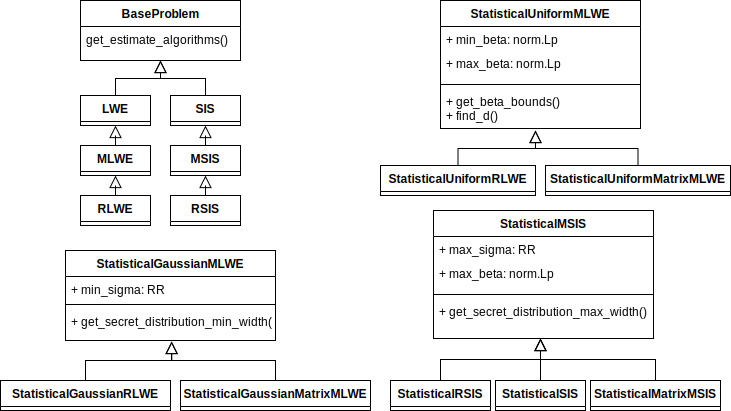
\includegraphics[width=0.8\textwidth]{../thesis/graphics/problem_classes.pdf}
\end{frame}

\section{Norms and Distributions}
\begin{frame}
    \frametitle{Norms and Distributions}
    \begin{itemize}[<+->]
        \item Classes \texttt{norm.Lp} and \texttt{norm.Cp} for $\ell_p$-norms and norms on the canonical embedding respectively
        \item Norm bounding in class methods \texttt{to\_Lp()}, addition and multiplication supported
        \item Uniform and Gaussian distribution and Gaussian to bound in module $\texttt{distributions}$
    \end{itemize}
\end{frame}

\SetKwInOut{KwInput}{Input}

\section{Generic Parameter Search}
\begin{frame}
    \frametitle{Main functionality}
    \begin{algorithm2e}[H]
        \KwInput{sec, initial\_params, next\_parameters, parameter\_cost,  problem\_instance}
        \pause
        L = OrderedList(initial\_params)\\\pause
        \While{L $\neq \emptyset$}{
            current\_params = L.pop() \\
            instances = parameter\_problem(current\_params) \\\pause
            result = estimate(instances, sec) \\
            \If{result is secure}{
                \Return{(result, current\_params)}\\
            }\pause
            \Else{
                next\_param\_sets = next\_parameters(current\_params)\\
                \ForAll{param\_set in next\_param\_sets}{
                    sort param\_set into L according to parameter\_cost function\\
                }
            }
        }
        \caption{Generic Search}
    \end{algorithm2e}
\end{frame}

\section{Demo}

\begin{frame}[c]{}
    \centering \Huge
    \emph{Thank You!}
\end{frame}
% \begin{frame}
%     \frametitle{TODO}
%     \begin{itemize}
%         \item<1-> Text visible on slide 1
%         \item<2-> Text visible on slide 2
%     \end{itemize}
%     \begin{block}{Test}
%         Test
%     \end{block}
%     \begin{alertblock}{Test}
%         Test
%     \end{alertblock}
%     \begin{examples}{Test}
%         Test
%     \end{examples}

% \end{frame}

% \begin{frame}
%     \frametitle{Two-column slide}
%     \begin{columns}
%         \column{0.5\textwidth}
%         This is a text in first column.
%         $$E=mc^2$$
%         \begin{itemize}
%             \item First item
%             \item Second item
%         \end{itemize}

%         \column{0.5\textwidth}
%         This text will be in the second column
%         and on a second thoughts, this is a nice looking
%         layout in some cases.
%     \end{columns}
% \end{frame}

\begin{frame}[allowframebreaks]
    \frametitle{References}
    % This prints the bibliography on the slide
    \printbibliography
\end{frame}








%%%%%%%%%%%%%%%%%%%%%%%%%%%%%%%%%%%%%%%%%%%%%%%
% Additional
%%%%%%%%%%%%%%%%%%%%%%%%%%%%%%%%%%%%%%%%%%%%%%%
%%%%%%%%%%%%%%%%%%%%%%%%%%%%%%%%%%%%%%%%%%%%%%%
%%%%%%%%%%%%%%%%%%%%%%%%%%%%%%%%%%%%%%%%%%%%%%%
%%%%%%%%%%%%%%%%%%%%%%%%%%%%%%%%%%%%%%%%%%%%%%%
%%%%%%%%%%%%%%%%%%%%%%%%%%%%%%%%%%%%%%%%%%%%%%%
\begin{frame}
    \frametitle{Gram-Schmidt Orthogonalization}
    \begin{itemize}[<+->]
        \item Given basis $\mathbf{B} = \left[\mathbf{b}_1 \cdots \mathbf{b}_n\right]$
        \item Define $\tilde{\mathbf{b}}_i$ as follows:
              \begin{itemize}
                  \item $\tilde{\mathbf{b}}_1 = \mathbf{b}_1$
                  \item For $i \in \{2, \ldots, n\}$:
                        \begin{equation*}
                            \tilde{\mathbf{b}}_i = \mathbf{b}_i - \pi_{\text{span}(\mathbf{b}_1, \ldots, \mathbf{b}_{i-1})}(\mathbf{b}_i).
                        \end{equation*}
              \end{itemize}
        \item $\tilde{\mathbf{B}} = \left[\tilde{\mathbf{b}}_1 \cdots \tilde{\mathbf{b}}_n\right]$ is the Gram-Schmidt orthogonalization of $\mathbf{B}$
        \item We define Gram-Schmidt coefficients
              \begin{equation*}
                  \mu_{i, j} = \frac{\left\langle \tilde{\mathbf{b}}_j, \mathbf{b}_i\right\rangle}{\left\langle \tilde{\mathbf{b}}_j, \tilde{\mathbf{b}}_j\right\rangle}
              \end{equation*}
    \end{itemize}
\end{frame}
\begin{frame}
    \frametitle{The LLL Algorithm}
    \begin{itemize}[<+->]
        \item Proposed by Lenstra, Lenstra and Lovász in \only<.->{\footfullcite{LLL82}} %TODO: could add more details
        \item Finds short vectors of length at most $2^{n/2} \lambda_1(\Lambda)$ in polynomial time % TODO: say lambda_1 is shortest lattice vector
        \item A $\theta$-LLL reduced basis ensures two criteria:
              \begin{itemize}[<+->]
                  \item Size-reduced: $|\mu_{i,j}| \leq \frac{1}{2}$ for $1\leq i \leq n$ and $j < i$
                  \item Lovász condition: $\theta \| \tilde{\mathbf{b}}_i \|^2 > \| \mu_{i+1, i} \tilde{\mathbf{b}}_i + \tilde{\mathbf{b}}_{i+1} \|^2$ for $1\leq i < n$
              \end{itemize}
    \end{itemize}
\end{frame} % TODO: output quality?

\begin{frame}
    \frametitle{The LLL Algorithm}
    \begin{algorithm2e}[H]
        \SetKwBlock{Begin}{function}{end function}
        \Begin($\theta\text{-LLL} {(}\mathbf{B} \in \mathbb{Z}^{m\times n} {)}$)
        {
            Compute $\tilde{\mathbf{B}}$\label{alg:LLL-start}\\\pause
            \For{$i=2, \dots, n$}{
                \For{$j=i-1, \dots, 1$}{
                    $\mathbf{b}_i = \mathbf{b}_i - \lfloor\mu_{i, j}\rceil \mathbf{b}_j$\label{alg:LLL-red}\\
                }
            }\pause
            \If{$\exists i \text{ \upshape such that } \theta \| \tilde{\mathbf{b}}_i \|^2 > \| \mu_{i+1, i} \tilde{\mathbf{b}}_i + \tilde{\mathbf{b}}_{i+1} \|^2$}{
                Swap $\mathbf{b}_{i}$ and $\mathbf{b}_{i+1}$\label{alg:LLL-swap}\\
                Return $\theta$-LLL($\mathbf{B}$)\\
            }
            \Else{
                Return $\mathbf{B}$\\
            }
        }
        \caption{The LLL Algorithm\footfullcite{LLLReg04}} \label{alg:LLL}
    \end{algorithm2e}
\end{frame}

\begin{frame}
    \frametitle{The Block Korkin-Zolatarev (BKZ) Algorithm\footfullcite{SE91}}
    \begin{itemize}[<+->]
        \item LLL reduce input basis $\left\{\mathbf{b}_1, \dots, \mathbf{b}_{n}\right\}$
        \item In $j$th iteration project block $\mathbf{b}_j, \dots, \mathbf{b}_{j+k-1}$ to the orthogonal complement of $\text{span}\left(\left\{\mathbf{b}_i \mid i \in [j-1]\right\}\right)$ % TODO: be able to explain orthogonal complement
        \item Run SVP oracle on the projected block to obtain shortest vector $\mathbf{b}_\text{new}'$ in the projected lattice
        \item Recover lattice vector $\mathbf{b}_\text{new}$ from $\mathbf{b}_\text{new}'$
        \item If $\mathbf{b}_\text{new}$ is new, insert $\mathbf{b}_\text{new}$ into list of basis vectors and run LLL on $\{\mathbf{b}_j, \dots, \mathbf{b}_{j-1}, \mathbf{b}_\text{new}, \mathbf{b}_j, \dots, \mathbf{b}_{h} \}$ to obtain $n$ linearly independent basis vectors
        \item Repeat until no change in $n$ iterations, counter $j$ resets to $1$ after $n-k+1$ iterations (one round)
    \end{itemize}
\end{frame}
\begin{frame}
    \frametitle{BKZ}
    \begin{itemize}[<+->]
        \item Various improvements: early termination, local preprocessing, progressive BKZ
        \item Simplified runtime estimate: $\rho \cdot n \cdot t_k$
              \begin{itemize}
                  \item $\rho$: number of rounds
                  \item $t_k$: cost of SVP oracle in dimension $k$
              \end{itemize}
        \item Most significant progress in first $8$ rounds\only<.->{\footfullcite{Chen13}} $\Rightarrow$ LWE-Estimator chooses $\rho = 8$
    \end{itemize} % TODO: what about output quality?
\end{frame}


\begin{frame}
    \frametitle{Primal Attack - Reduction of LWE to BDD}
    \begin{block}{BDD$_\gamma$}
        Given a lattice $\Lambda \subset \mathbb{R}^m$ and a target vector $\mathbf{t}\in\mathbb{R}^m$ such that $\text{dist}(\mathbf{t}, \Lambda) < \gamma \lambda_1(\Lambda)$, the (approximate)  Bounded Distance Decoding (BDD$_\gamma$) is the problem of finding the closest lattice vector $\mathbf{v} \in \Lambda$, i.e., $\mathbf{v} = \argmin_{\mathbf{v}' \in \Lambda} \|\mathbf{v}' - \mathbf{t}\|$.
    \end{block}\pause
    Consider the LWE lattice $\Lambda_q(\mathbf{A}^\intercal) = \left\{ \mathbf{v} \in \mathbb{Z}^m \mid \exists \mathbf{y} \in \mathbb{Z}^n : \mathbf{v} = \mathbf{A}^\intercal \mathbf{y} \mod q \right\}$.\pause
    \begin{itemize}[<+->]
        \item $\mathbf{z} = \mathbf{A}^\intercal \mathbf{s} + \mathbf{e} \mod q = \mathbf{A}^\intercal \mathbf{s} + \mathbf{e} + q \mathbf{x}$ for some $\mathbf{x} \in \mathbb{Z}^m$
        \item $\mathbf{A}^\intercal \mathbf{s} + q \mathbf{x}$
        \item $\text{dist}(\mathbf{z}, \Lambda_q(\mathbf{A}^\intercal) = \|\mathbf{e}\|$ and, in general, $\|\mathbf{e}\| < \gamma \lambda_1(\Lambda_q(\mathbf{A}^\intercal))$ % TODO explain distance
        \item Solving BDD solves LWE
    \end{itemize}
\end{frame}
\begin{frame}
    \frametitle{Primal Attack - Variants}
    \begin{itemize}[<+->]
        \item Decoding Attack\footfullcite{LP11}
              \begin{itemize}[<+->]
                  \item Reduction step: run BKZ to improve basis quality
                  \item Decoding step: run a generalized variant of Babai's Nearest Planes (GNP) algorithm to enumerate candidate lattice vectors% TODO: include this variant?
                  \item Choose parameters for BKZ and GNP such that $t_{\text{DEC}} = \rho\cdot (t_{\text{BKZ}} + t_{\text{GNP}})$ is minimized % TODO: note that \rho depends on required output success probability            
              \end{itemize}
    \end{itemize}
\end{frame}
\begin{frame}
    \frametitle{Primal Attack - Variants}
    \begin{itemize}[<+->]
        \item Primal uSVP \only<.->{\footfullcite{AFG13}}
              \begin{itemize}[<+->]
                  \item Embed LWE lattice $\Lambda(\mathbf{B})$ in a new lattice $\Lambda(\mathbf{B}')$ with uSVP structure % explain usvp or (i.e., $\exists \gamma > 1: \lambda_2(\Lambda) > \gamma \lambda_1(\Lambda)$)
                        \begin{equation*}
                            \mathbf{B}' = \begin{pmatrix}
                                \mathbf{B}           & \mathbf{z} \\
                                \mathbf{0}^\intercal & \mu
                            \end{pmatrix}
                        \end{equation*}
                  \item Unique shortest vector in $\Lambda'$ is $\mathbf{z}' = \left[-\mathbf{e}^\intercal, -\mu\right]^\intercal$ for some $\mu$ % in practice \mu = 1$
                  \item Run BKZ to find $\mathbf{z}'$ and recover $\mathbf{s}$ % TODO: determine necessary root hermite factor => block size k, tradeoff success probability and rounds
              \end{itemize}
    \end{itemize}
\end{frame}

\begin{frame}
    \frametitle{Reduction of LWE to SIS\footfullcite{LP11}}
    \begin{itemize}[<+->]
        \item Consider the dual SIS lattice $\Lambda_q(\mathbf{A}^\intercal)^{\perp} = \{ \mathbf{y} \in \mathbb{Z}^m \mid \mathbf{A} \mathbf{y} = \mathbf{0} \mod q\}$
        \item For a lattice vector $\mathbf{v} \in \Lambda_q(\mathbf{A}^\intercal)^{\perp}$ it holds that
              \begin{align*}
                  \langle \mathbf{v}, \mathbf{z} \rangle & = \langle \mathbf{v}, \mathbf{A}^\intercal \mathbf{s} \rangle + \langle \mathbf{v}, \mathbf{e}\rangle = \langle \mathbf{v}\mathbf{A}^\intercal,  \mathbf{s} \rangle + \langle \mathbf{v}, \mathbf{e} \rangle \\
                                                         & = \langle \mathbf{v}, \mathbf{e} \rangle \mod q
              \end{align*}
        \item Test whether $\langle \mathbf{v}, \mathbf{e} \rangle \mod q$ corresponds to Gaussian of width $\|\mathbf{v}\| \cdot s$ % e is distributed according to gaussian of width s
        \item Advantage is close to $\exp(-\pi (\| \mathbf{v} \| s/q)^2)$
        \item Finding a short non-zero vector $\mathbf{v}$ in the dual SIS lattice solves Decision-LWE
    \end{itemize} % TODO
\end{frame}
\begin{frame}
    \frametitle{The Blum, Kalai and Wassermann (BKW) Algorithm\footfullcite{BKW03}}
    \begin{itemize}[<+->]
        \item Reduce dimension of input matrix $\mathbf{A}$ by finding collisions of its column vectors
        \item In each step eliminate $b$ components of the samples
              \begin{itemize}[<+->]
                  \item $z_i = \left\langle \mathbf{a}_i \mathbf{s}\right\rangle + e_i$ and $z_j = \left\langle \mathbf{a}_j \mathbf{s}\right\rangle + e_j$ where $\mathbf{a}_i$ and $\mathbf{a}_j$ match in the last $b$ components
                  \item $\mathbf{a}_i - \mathbf{a}_j$ has only zero entries in the last $b$ components
                  \item $z_i - z_j = \left\langle \mathbf{a}_i - \mathbf{a}_j\right\rangle + e_i - e_j$
              \end{itemize}
        \item Repeat $a$ times until only small number of components left
        \item Recover secret vector by means of hypothesis testing and back substitution
        \item Runtime complexity $\approx \left(a^2 n\right) \cdot \frac{q^b}{2}$ % a,b depend on n, q, alpha, TODO: why the complexity?
        \item Estimator uses a variant called Coded-BKW% TODO: cite??? -> more space on slide needed
    \end{itemize}
\end{frame}

\begin{frame}
    \frametitle{Other Approaches}
    \begin{itemize}[<+->]
        \item Exhaustive search: Meet-In-The-Middle attack
        \item Arora-GB: solve system of non-linear equations
        \item In practice much slower than other algorithms
    \end{itemize}
\end{frame}

\begin{frame}
    \frametitle{Solving SIS - Dual Attack\footfullcite{MR09}}% TODO
    \begin{itemize}[<+->]
        \item Finding short vector $\mathbf{v} \in \Lambda(\mathbf{A}^\intercal)^{\perp}$ with $\|\mathbf{v}\| \leq \beta$ in the dual SIS lattice solves SIS
        \item Lattice reduction yields $\mathbf{b}_1$ of length length $\|\mathbf{b}_1\| = \delta^m q^{n/m}$ (under the assumption that $\text{det}(\Lambda(\mathbf{A}^\intercal)^{\perp})\approx q^n$) % say: we see that delta depends on m
        \item Optimal subdimension is $m' = \sqrt{\frac{n \log q}{\log \delta}}$ % that's where the expression in the previous point becomes minimal
        \item Log root Hermite Factor for optimal subdimension is
              \begin{equation*}
                  \log \delta = \frac{\log^2 \beta}{4n \log q}
              \end{equation*}
        \item Similar result in Rückert and Schneider (2010, IACR Cryptol. ePrint Arch.)
    \end{itemize}
\end{frame}
\begin{frame}
    \frametitle{Solving SIS - Combinatorial Attack\footfullcite{MR09}}% TODO
    \begin{itemize}[<+->]
        \item Find $\mathbf{v} \in \Lambda(\mathbf{A}^\intercal)^{\perp}$ with coefficients bounded by $\beta$, i.e., $\|\mathbf{v}\|_\infty \leq \beta$
        \item Divide columns of $\mathbf{A}$ into $2^k$ sets of $m/2^k$ vectors
        \item Compute a new set of all linear combinations of the vectors for each set with coefficients bounded by $\beta$
        \item[$\Rightarrow$] $L=(2\beta+1)^{m/2^k}$ vectors per set
        \item In each step pairwise combine vectors of two sets such that $\log_q L$ components are eliminated
              %\item Choose $k$ such that  $n \approx (k+1) \log_q L$ %by minimizing
              %   \begin{align*}
              %       \Delta & = \text{abs}\left(\frac{2^k}{k+1} - \frac{m \log(2\beta + 1)}{n \log(q)}\right)
              %   \end{align*}
        \item Overall cost dominated by list size $L$, total cost $\approx 2^k \cdot L \cdot \log_2(q) \cdot n$ % explain: number of lists, list size, ops
    \end{itemize}
\end{frame}




\begin{frame}
    \frametitle{Ring-SIS}
    \begin{block}{RSIS}
        Let $\mathcal{R}_q$ be the quotient ring $\mathbb{Z}_q\left[x\right] / \left\langle x^n + 1 \right\rangle$. Given $a_1, \ldots, a_m \in \mathcal{R}_q$ chosen independently from the uniform distribution, the Ring-SIS problem RSIS$_{n, q, m, \beta}$ asks to find $s_1, \ldots, s_m \in \mathcal{R}$ such that $\sum_{i=1}^m \mathbf{a}_i \cdot s_i = 0 \mod q$ and $0 < \| \mathbf{s}\| \leq \beta$, where $\mathbf{s} = \left[s_1, \ldots, s_m\right]^\intercal \in \mathcal{R}^m$.
    \end{block}
    \pause
    \begin{itemize}[<+->]
        \item Interpret $r \in \mathcal{R}$ as an $n$ dimensional vector s.t. $r = \sum_{i=0}^{n-1} r_i x^i$
        \item Each $a_i$ in RSIS corresponds to an $n\times n$ block in the standard SIS matrix $\mathbf{A}_\text{SIS}$ obtained by rotation:
              \begin{equation*}
                  \text{Rot}(a) = \begin{pmatrix}
                      a_0     & -a_{n-1} & \cdots & -a_{1} \\
                      a_1     & a_{0}    & \cdots & -a_{2} \\
                      \vdots  & \vdots   & \ddots & \vdots \\
                      a_{n-1} & a_{n-2}  & \cdots & a_{0}  \\
                  \end{pmatrix}
              \end{equation*}
        \item[$\Rightarrow$] $\mathbf{A}_\text{SIS} = [\text{Rot}(a_1)\mid \dots \mid \text{Rot}(a_m)]$
        \item RSIS$_{n, q, m, \beta} \longrightarrow$ SIS$_{n, q, m \cdot n, \beta}$
    \end{itemize}
\end{frame}

\begin{frame}[t]
    \frametitle{Module-SIS}
    \begin{block}{MSIS}
        Let $\mathcal{R}^d$ be a module with ring dimension $n$ and module rank $d$. Given  $\mathbf{a}_1, \ldots, \mathbf{a}_m \in \mathcal{R}_q^d$ chosen independently from the uniform distribution, the Module-SIS problem \text{MSIS}$_{n, d, q, m, \beta}$ asks to find $s_1, \ldots, s_m \in \mathcal{R}$ such that $\sum_{i=1}^m \mathbf{a}_i \cdot s_i = \mathbf{0}\mod q$ and $0 < \| \mathbf{s}\| \leq \beta$, where $\mathbf{s} = \left[s_1, \ldots, s_m\right]^\intercal \in \mathcal{R}^m$.
    \end{block} \pause % TODO: quotient ring
    \only<2>{\begin{itemize}
            \item Module element $\mathbf{a}_i$ corresponds to $n\cdot d \times n$ block in $\mathbf{A}$ and for $\mathbf{A}$ can be viewed as a $n\cdot d \times n \cdot m$ matrix
        \end{itemize}}

    \only<3>{
        \begin{center}
            \includegraphics[width=0.35\textwidth]{../thesis/graphics/MSIS_matrix.pdf}
        \end{center}}

    \only<4->{\begin{itemize}
            \item Module element $\mathbf{a}_i$ corresponds to $n\cdot d \times n$ block in $\mathbf{A}$ and for $\mathbf{A}$ can be viewed as a $n\cdot d \times n \cdot m$ matrix
            \item MSIS$_{n, d, q, m, \beta} \longrightarrow$ SIS$_{n \cdot d, q, m \cdot n, \beta}$
        \end{itemize}}
\end{frame}
\begin{frame}
    \frametitle{Ring-LWE and Module-LWE}
    \begin{block}{RLWE Distribution}
        Let $\chi$ be the error distribution on $\mathbb{T}_{\mathcal{R}^\perp} = K_\mathbb{R} / \mathcal{R}^\perp$ and $s \in \mathcal{R}^\perp$ be the secret. Then, we define $\mathcal{A}_{q, s, \chi}^{(\mathcal{R})}$ as the Ring-LWE (RLWE) distribution on $\mathcal{R}_q \times \mathbb{T}_{\mathcal{R}^\perp}$ obtained by choosing $a \in \mathbb{R}_q$ uniformly at random and an error term $e \in \mathbb{T}_{\mathcal{R}^\perp}$ according to $\chi$, and returning samples $(a, (a \cdot s)/q + e)$.
    \end{block}\pause
    \begin{block}{MLWE Distribution}
        Let $\chi$ be the error distribution on $\mathbb{T}_{\mathcal{R}^\perp}$ and $\mathbf{s} \in (\mathcal{R}^\perp)^d$ be the secret vector. Then, we define $\mathcal{A}_{q, \mathbf{s}, \chi}^{(\mathcal{M})}$ as the Module-LWE (MLWE) distribution on $(\mathcal{R}_q)^d \times \mathbb{T}_{\mathcal{R}^\perp}$ obtained by choosing $\mathbf{a} \in (\mathbb{R}_q)^d$ uniformly at random and an error term $e \in \mathbb{T}_{\mathcal{R}^\perp}$ according to $\chi$, and returning samples $(\mathbf{a}, \frac{1}{q}\langle \mathbf{a},\mathbf{s}\rangle + e)$.
    \end{block}
    \begin{itemize}[<+->]
        \item RLWE$_{n, q, m, \chi} \longrightarrow$ LWE$_{n, q, m \cdot n, \chi}$
        \item MLWE$_{n, d, q, m, \chi} \longrightarrow$ LWE$_{n \cdot d, q, m \cdot n, \chi}$
    \end{itemize}
\end{frame}

\begin{frame}
    \frametitle{Statistically Secure MLWE (Gaussian Variant)\footfullcite{LPR13}}
    \begin{itemize}[<+->]
        \item Given $m$th cyclomatic number field $K$ of degree $n=\phi(m)$ and integer $q\geq 2$ and
        \item $\mathbf{A} = [ \mathbf{I}_{[m]} \mid \bar{\mathbf{A}}] \in (\mathcal{R}_q)^{[m] \times [m+d]}$ with positive integers $m \leq m + d \leq \text{poly}(n)$ and uniformly random matrix $\bar{\mathbf{A}}$ % TODO: explain A
        \item Let $\mathbf{x} \in (\mathcal{R}_q)^{[m+d]}$ where each component is chosen from a discrete Gaussian distribution of parameter $s > 2n \cdot q^{m / (m+d) + 2/(n (m+d))}$ over $\mathcal{R}$
        \item Then $\mathbf{A}\mathbf{x} \in (\mathcal{R}_q)^{[m]}$ is within statistical distance $2^{-\Omega(n)}$ of the uniform distribution over $(\mathcal{R}_q)^{[m]}$)
              % TODO: explain how Ax is LWE... how we can call these...
              % Also works for RLWE
    \end{itemize}
\end{frame}

\begin{frame}
    \frametitle{Statistically Secure MLWE (Uniform Variant)\footfullcite{BDLOP18}}
    \begin{itemize}[<+->]
        \item Given $\mathbf{A} = [ \mathbf{I}_{[m]} \mid \bar{\mathbf{A}}] \in (\mathcal{R}_q)^{[m] \times [m+d]}$ as before, $1 < d_2 < n$, where $d_2$ is a power of 2 and a prime $q$ congruent to $2d_2 + 1 \;(\text{mod } 4d_2)$
        \item If $\beta\in \mathbb{R}$ such that $\beta_{min} \leq \beta \leq \beta_{max}$ with
              \begin{align*}
                  \beta_{min} & = \frac{q^{m/(m+d)} \cdot 2^{2 \texttt{sec}/((m+d)\cdot n)}}{2} \\
                  \beta_{max} & = \frac{1}{2\sqrt{d_2}} \cdot q^{1/d_2} - 1
              \end{align*}\pause
              then  any (all-powerful) algorithm $\mathcal{A}$ has advantage at most $2^{-\texttt{sec}}$ in distinguishing $\mathbf{A}\mathbf{x} \in (\mathcal{R}_q)^{[m]}$ from the uniform distribution, where $\mathbf{x}$ is chosen uniformly random with $\|\mathbf{x}\|_\infty \leq \beta$
              % Also works for RLWE
    \end{itemize}
\end{frame}
\begin{frame}
    \frametitle{Statistical MSIS\footfullcite{DOTT21}}
    \begin{itemize}[<+->]
        \item Given $\mathbf{A} = [ \mathbf{I}_{[m]} \mid \bar{\mathbf{A}}] \in (\mathcal{R}_q)^{[m] \times [m+d]}$ as before
        \item It should be hard to find $\mathbf{r}, \mathbf{r}' \in \mathcal{R}_q^{m+d}$ of $\ell_2$-norm $\leq B$ such that $\mathbf{A} \cdot (\mathbf{r} - \mathbf{r}') = \mathbf{0} \text{ mod } q$
        \item We demand that $\text{Pr}[\mathbf{A} \cdot \mathbf{r} = \mathbf{0}] \leq 2^{- \texttt{sec}}$ with non zero elements $\mathbf{r}$ in the Euclidean ball $B_{m}(0, 2B)$
        \item Satisfied if
              \begin{equation*}
                  B \leq 2^{\frac{-\texttt{sec}}{(m+d)\cdot n} - 1} \cdot q^\frac{m}{m+d} \cdot \sqrt{\frac{(m+d)\cdot n}{2 \pi e}}
              \end{equation*}
        \item Also works for RSIS and SIS
    \end{itemize}
\end{frame}



\begin{frame}
    \frametitle{Norm Bounding}
    Let $f \in \mathcal{R}_q$  with $f = \sum_i f_i X^i$ and $\sigma : K \rightarrow \mathbb{C}$ with number field $K$ the canonical embedding\footfullcite{BDLOP18,DPSZ12} and $p, q \in \mathbb{N}$.\pause
    \begin{itemize}[<+->]
        \item $\| f \|_p \leq \| f \|_q$, for $\infty \geq p \geq q \geq 1$
        \item $\lim_{q' \rightarrow q}\| f \|_p \leq \lim_{q' \rightarrow q} n^{\frac{1}{p} - \frac{1}{q'}}\| f \|_{q'}$ for $1 \leq p \leq q \leq \infty$
        \item $\| \sigma(f) \|_\infty\leq \| f \|_1 \leq n^{1 - \frac{1}{p}} \| f \|_p $ for $p \geq 1$
        \item $\| f \|_p             \leq  n^{\frac{1}{p}} \| f \|_\infty \leq n^{\frac{1}{p}} \| \sigma(f) \|_\infty$ for  $p \leq \infty$
    \end{itemize}
\end{frame}
\begin{frame}
    \frametitle{Norm Bounding}
    Let $f \in \mathcal{R}_q$  with $f = \sum_i f_i X^i$ and $\sigma : K \rightarrow \mathbb{C}$ with number field $K$ the canonical embedding\footfullcite{BDLOP18,DPSZ12} and $p, q \in \mathbb{N}$.\pause
    \begin{itemize}[<+->]
        \item $\|f \cdot g\|_\infty \leq \|f\|_\infty \cdot \|g\|_1$
        \item $\|f \cdot g\|_\infty \leq \|f\|_2 \cdot \|g\|_2$
        \item $\| \sigma(x \cdot y) \|_p \leq  \| \sigma(x) \|_\infty \cdot \| \sigma(y) \|_p$
        \item Encapsulated in $\texttt{to\_Lp()}$ and $\texttt{to\_Cp()}$ of the norm classes $\texttt{Lp}$ and $\texttt{Cp}$
    \end{itemize}
\end{frame}

\begin{frame}
    \frametitle{Gaussian to Bound} % perhaps only to bound relevant?
    \begin{itemize}[<+->]
        \item Classes for uniform and Gaussian distribution in the module $\texttt{distributions}$
        \item Gaussian
              \begin{itemize}[<+->]
                  \item Constructors for standard deviation $\sigma$, $s =\sigma \sqrt{2 \pi}$, and $\alpha = \frac{s}{q} = \frac{\sqrt{2\pi} \sigma}{q}$
                  \item Gaussian to bound conversion\footfullcite{Lyu12}
                        \begin{itemize}[<+->]
                            \item For $\ell_\infty$-norm:
                                  \begin{equation*}
                                      \beta  = s \sqrt{\frac{(\texttt{sec} + 1) \ln(2)}{\pi}}
                                  \end{equation*}
                            \item For $\ell_2$-norm:
                                  \begin{equation*}
                                      \text{Pr}\left[ \|X\|_2 > \sigma \sqrt{2n} \right] \leq 2^{\frac{n}{2}(1 -\log e)}
                                  \end{equation*}
                            \item[$\Rightarrow$] Set $\beta = \sigma \sqrt{2n}$, if $2^{\frac{n}{2}(1 -\log e)} \leq 2^{-\texttt{sec}}$
                            \item In all other cases $\texttt{to\_Lp()}$ bounds the value via $\ell_2$-norm
                        \end{itemize}
              \end{itemize}
    \end{itemize}
\end{frame}




\end{document}